\documentclass[twoside]{book}

% Packages required by doxygen
\usepackage{calc}
\usepackage{doxygen}
\usepackage{graphicx}
\usepackage[utf8]{inputenc}
\usepackage{makeidx}
\usepackage{multicol}
\usepackage{multirow}
\usepackage{fixltx2e}
\PassOptionsToPackage{warn}{textcomp}
\usepackage{textcomp}
\usepackage[nointegrals]{wasysym}
\usepackage[table]{xcolor}

% Font selection
\usepackage[T1]{fontenc}
\usepackage{mathptmx}
\usepackage[scaled=.90]{helvet}
\usepackage{courier}
\usepackage{amssymb}
\usepackage{sectsty}
\renewcommand{\familydefault}{\sfdefault}
\allsectionsfont{%
  \fontseries{bc}\selectfont%
  \color{darkgray}%
}
\renewcommand{\DoxyLabelFont}{%
  \fontseries{bc}\selectfont%
  \color{darkgray}%
}
\newcommand{\+}{\discretionary{\mbox{\scriptsize$\hookleftarrow$}}{}{}}

% Page & text layout
\usepackage{geometry}
\geometry{%
  a4paper,%
  top=2.5cm,%
  bottom=2.5cm,%
  left=2.5cm,%
  right=2.5cm%
}
\tolerance=750
\hfuzz=15pt
\hbadness=750
\setlength{\emergencystretch}{15pt}
\setlength{\parindent}{0cm}
\setlength{\parskip}{0.2cm}
\makeatletter
\renewcommand{\paragraph}{%
  \@startsection{paragraph}{4}{0ex}{-1.0ex}{1.0ex}{%
    \normalfont\normalsize\bfseries\SS@parafont%
  }%
}
\renewcommand{\subparagraph}{%
  \@startsection{subparagraph}{5}{0ex}{-1.0ex}{1.0ex}{%
    \normalfont\normalsize\bfseries\SS@subparafont%
  }%
}
\makeatother

% Headers & footers
\usepackage{fancyhdr}
\pagestyle{fancyplain}
\fancyhead[LE]{\fancyplain{}{\bfseries\thepage}}
\fancyhead[CE]{\fancyplain{}{}}
\fancyhead[RE]{\fancyplain{}{\bfseries\leftmark}}
\fancyhead[LO]{\fancyplain{}{\bfseries\rightmark}}
\fancyhead[CO]{\fancyplain{}{}}
\fancyhead[RO]{\fancyplain{}{\bfseries\thepage}}
\fancyfoot[LE]{\fancyplain{}{}}
\fancyfoot[CE]{\fancyplain{}{}}
\fancyfoot[RE]{\fancyplain{}{\bfseries\scriptsize Generated on Thu Jul 17 2014 21\+:08\+:39 for T\+F\+T Touch Screen Strings by Doxygen }}
\fancyfoot[LO]{\fancyplain{}{\bfseries\scriptsize Generated on Thu Jul 17 2014 21\+:08\+:39 for T\+F\+T Touch Screen Strings by Doxygen }}
\fancyfoot[CO]{\fancyplain{}{}}
\fancyfoot[RO]{\fancyplain{}{}}
\renewcommand{\footrulewidth}{0.4pt}
\renewcommand{\chaptermark}[1]{%
  \markboth{#1}{}%
}
\renewcommand{\sectionmark}[1]{%
  \markright{\thesection\ #1}%
}

% Indices & bibliography
\usepackage{natbib}
\usepackage[titles]{tocloft}
\setcounter{tocdepth}{3}
\setcounter{secnumdepth}{5}
\makeindex

% Hyperlinks (required, but should be loaded last)
\usepackage{ifpdf}
\ifpdf
  \usepackage[pdftex,pagebackref=true]{hyperref}
\else
  \usepackage[ps2pdf,pagebackref=true]{hyperref}
\fi
\hypersetup{%
  colorlinks=true,%
  linkcolor=blue,%
  citecolor=blue,%
  unicode%
}

% Custom commands
\newcommand{\clearemptydoublepage}{%
  \newpage{\pagestyle{empty}\cleardoublepage}%
}


%===== C O N T E N T S =====

\begin{document}

% Titlepage & ToC
\hypersetup{pageanchor=false,
             bookmarks=true,
             bookmarksnumbered=true,
             pdfencoding=unicode
            }
\pagenumbering{roman}
\begin{titlepage}
\vspace*{7cm}
\begin{center}%
{\Large T\+F\+T Touch Screen Strings }\\
\vspace*{1cm}
{\large Generated by Doxygen 1.8.7}\\
\vspace*{0.5cm}
{\small Thu Jul 17 2014 21:08:39}\\
\end{center}
\end{titlepage}
\clearemptydoublepage
\tableofcontents
\clearemptydoublepage
\pagenumbering{arabic}
\hypersetup{pageanchor=true}

%--- Begin generated contents ---
\chapter{Main Page}
\label{index}\hypertarget{index}{}\hypertarget{index_intro_sec}{}\section{Introduction}\label{index_intro_sec}
\begin{DoxyAuthor}{Author}
Richard Kirkpatrick 
\end{DoxyAuthor}
\begin{DoxyDate}{Date}
17 July 2014 
\end{DoxyDate}
\begin{DoxyCopyright}{Copyright}
G\+N\+U Public License.
\end{DoxyCopyright}
This is the Arduino library for creating geometries shapes for the Seeed Studio T\+F\+T touch screen (Version 1). The user can create polygons, rectangles, triangle and circles. See the Wiki documentation page for more info! 
\chapter{Hierarchical Index}
\section{Class Hierarchy}
This inheritance list is sorted roughly, but not completely, alphabetically\+:\begin{DoxyCompactList}
\item \contentsline{section}{Touch\+Screen\+Text}{\pageref{class_touch_screen_text}}{}
\begin{DoxyCompactList}
\item \contentsline{section}{Touch\+Screen\+Char}{\pageref{class_touch_screen_char}}{}
\item \contentsline{section}{Touch\+Screen\+String}{\pageref{class_touch_screen_string}}{}
\end{DoxyCompactList}
\end{DoxyCompactList}

\chapter{Class Index}
\section{Class List}
Here are the classes, structs, unions and interfaces with brief descriptions\+:\begin{DoxyCompactList}
\item\contentsline{section}{\hyperlink{class_button}{Button} \\*Abstract class for drawing rectangular buttons to the Seeed Studio T\+F\+T touch screen }{\pageref{class_button}}{}
\end{DoxyCompactList}

\chapter{Class Documentation}
\hypertarget{class_touch_screen_char}{\section{Touch\+Screen\+Char Class Reference}
\label{class_touch_screen_char}\index{Touch\+Screen\+Char@{Touch\+Screen\+Char}}
}


Subclass of \hyperlink{class_touch_screen_text}{Touch\+Screen\+Text}. Abstract class used for drawing char's to the touch screen.  




{\ttfamily \#include $<$Touch\+Screen\+Strings.\+h$>$}

Inheritance diagram for Touch\+Screen\+Char\+:\begin{figure}[H]
\begin{center}
\leavevmode
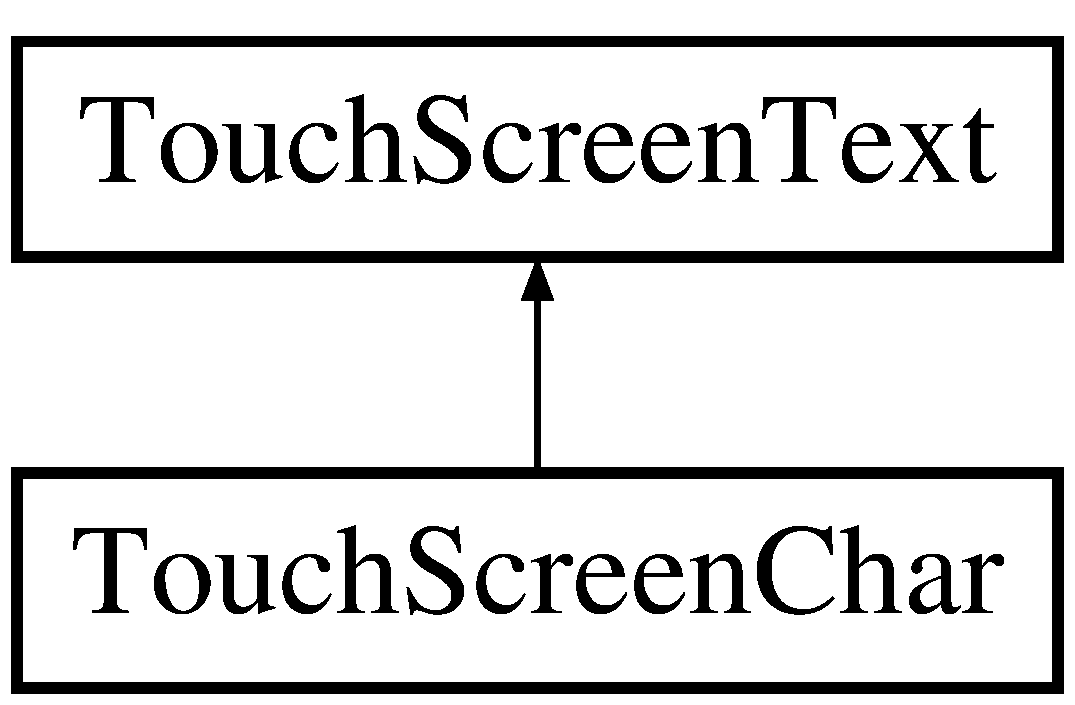
\includegraphics[height=2.000000cm]{class_touch_screen_char}
\end{center}
\end{figure}
\subsection*{Public Member Functions}
\begin{DoxyCompactItemize}
\item 
\hypertarget{class_touch_screen_char_a712dee575d947e58a776be559d33dc3f}{\hyperlink{class_touch_screen_char_a712dee575d947e58a776be559d33dc3f}{Touch\+Screen\+Char} ()}\label{class_touch_screen_char_a712dee575d947e58a776be559d33dc3f}

\begin{DoxyCompactList}\small\item\em Default constructor for the \hyperlink{class_touch_screen_string}{Touch\+Screen\+String} subclass. \end{DoxyCompactList}\item 
\hyperlink{class_touch_screen_char_a16271426fbf961392b6439c42c110c67}{Touch\+Screen\+Char} (\hyperlink{class_touch_screen_char}{Touch\+Screen\+Char} \&other\+Touch\+Screen\+Char)
\begin{DoxyCompactList}\small\item\em Copy constructor for the \hyperlink{class_touch_screen_string}{Touch\+Screen\+String} subclass. \end{DoxyCompactList}\item 
\hyperlink{class_touch_screen_char_a2a0a141a1d9b65b54031eea6317c2a63}{Touch\+Screen\+Char} (char my\+Text, int my\+X\+Start, int my\+Y\+Start, int my\+Font\+Size, unsigned int my\+Text\+Color)
\begin{DoxyCompactList}\small\item\em Parameter constructor for the \hyperlink{class_touch_screen_string}{Touch\+Screen\+String} superclass. \end{DoxyCompactList}\item 
void \hyperlink{class_touch_screen_char_a1cd1be7f6a6f0b7eefe198c70f799dce}{set\+Values} (char my\+Text, int my\+X\+Start, int my\+Y\+Start, int my\+Font\+Size, unsigned int my\+Text\+Color)
\begin{DoxyCompactList}\small\item\em Sets the char, cooordinates, font size, and char color. \end{DoxyCompactList}\item 
void \hyperlink{class_touch_screen_char_a3193c7b27aee874a21cdf86a39da6b61}{set\+Text} (char my\+Text)
\begin{DoxyCompactList}\small\item\em Sets the text of the char instance. \end{DoxyCompactList}\item 
const char \hyperlink{class_touch_screen_char_a14b7f8744d259592fe38522b131ca7c8}{get\+Text} ()
\begin{DoxyCompactList}\small\item\em Returns the char of the char instance. \end{DoxyCompactList}\item 
\hypertarget{class_touch_screen_char_a1c55410824b2adb0a480204366f9da01}{void \hyperlink{class_touch_screen_char_a1c55410824b2adb0a480204366f9da01}{draw\+Text} ()}\label{class_touch_screen_char_a1c55410824b2adb0a480204366f9da01}

\begin{DoxyCompactList}\small\item\em Uses the Seeed Studio library to draw the char. \end{DoxyCompactList}\item 
void \hyperlink{class_touch_screen_char_a099d277a6fc4510e93f02089070ca6f2}{text\+Button\+Display} ()
\begin{DoxyCompactList}\small\item\em Highlights the button text when pressed. \end{DoxyCompactList}\end{DoxyCompactItemize}
\subsection*{Additional Inherited Members}


\subsection{Detailed Description}
Subclass of \hyperlink{class_touch_screen_text}{Touch\+Screen\+Text}. Abstract class used for drawing char's to the touch screen. 

\subsection{Constructor \& Destructor Documentation}
\hypertarget{class_touch_screen_char_a16271426fbf961392b6439c42c110c67}{\index{Touch\+Screen\+Char@{Touch\+Screen\+Char}!Touch\+Screen\+Char@{Touch\+Screen\+Char}}
\index{Touch\+Screen\+Char@{Touch\+Screen\+Char}!Touch\+Screen\+Char@{Touch\+Screen\+Char}}
\subsubsection[{Touch\+Screen\+Char}]{\setlength{\rightskip}{0pt plus 5cm}Touch\+Screen\+Char\+::\+Touch\+Screen\+Char (
\begin{DoxyParamCaption}
\item[{{\bf Touch\+Screen\+Char} \&}]{other\+Touch\+Screen\+Char}
\end{DoxyParamCaption}
)}}\label{class_touch_screen_char_a16271426fbf961392b6439c42c110c67}


Copy constructor for the \hyperlink{class_touch_screen_string}{Touch\+Screen\+String} subclass. 


\begin{DoxyParams}{Parameters}
{\em other\+Touch\+Screen\+Char} & The char instance that is being copied. \\
\hline
\end{DoxyParams}
\hypertarget{class_touch_screen_char_a2a0a141a1d9b65b54031eea6317c2a63}{\index{Touch\+Screen\+Char@{Touch\+Screen\+Char}!Touch\+Screen\+Char@{Touch\+Screen\+Char}}
\index{Touch\+Screen\+Char@{Touch\+Screen\+Char}!Touch\+Screen\+Char@{Touch\+Screen\+Char}}
\subsubsection[{Touch\+Screen\+Char}]{\setlength{\rightskip}{0pt plus 5cm}Touch\+Screen\+Char\+::\+Touch\+Screen\+Char (
\begin{DoxyParamCaption}
\item[{char}]{my\+Text, }
\item[{int}]{my\+X\+Start, }
\item[{int}]{my\+Y\+Start, }
\item[{int}]{my\+Font\+Size, }
\item[{unsigned int}]{my\+Text\+Color}
\end{DoxyParamCaption}
)}}\label{class_touch_screen_char_a2a0a141a1d9b65b54031eea6317c2a63}


Parameter constructor for the \hyperlink{class_touch_screen_string}{Touch\+Screen\+String} superclass. 


\begin{DoxyParams}{Parameters}
{\em my\+Text} & The char that is to be drawn. \\
\hline
{\em my\+X\+Start} & The x-\/coordinate for the char instance. \\
\hline
{\em my\+Y\+Start} & The y-\/coordinate for the char instance. \\
\hline
{\em my\+Font\+Size} & The font size of the char instance. \\
\hline
{\em my\+Text\+Color} & The color of the char instance. \\
\hline
\end{DoxyParams}


\subsection{Member Function Documentation}
\hypertarget{class_touch_screen_char_a14b7f8744d259592fe38522b131ca7c8}{\index{Touch\+Screen\+Char@{Touch\+Screen\+Char}!get\+Text@{get\+Text}}
\index{get\+Text@{get\+Text}!Touch\+Screen\+Char@{Touch\+Screen\+Char}}
\subsubsection[{get\+Text}]{\setlength{\rightskip}{0pt plus 5cm}const char Touch\+Screen\+Char\+::get\+Text (
\begin{DoxyParamCaption}
{}
\end{DoxyParamCaption}
)}}\label{class_touch_screen_char_a14b7f8744d259592fe38522b131ca7c8}


Returns the char of the char instance. 

\begin{DoxyReturn}{Returns}
The char that is to be drawn. 
\end{DoxyReturn}
\hypertarget{class_touch_screen_char_a3193c7b27aee874a21cdf86a39da6b61}{\index{Touch\+Screen\+Char@{Touch\+Screen\+Char}!set\+Text@{set\+Text}}
\index{set\+Text@{set\+Text}!Touch\+Screen\+Char@{Touch\+Screen\+Char}}
\subsubsection[{set\+Text}]{\setlength{\rightskip}{0pt plus 5cm}void Touch\+Screen\+Char\+::set\+Text (
\begin{DoxyParamCaption}
\item[{char}]{my\+Text}
\end{DoxyParamCaption}
)}}\label{class_touch_screen_char_a3193c7b27aee874a21cdf86a39da6b61}


Sets the text of the char instance. 


\begin{DoxyParams}{Parameters}
{\em my\+Text} & The char that is to be drawn. \\
\hline
\end{DoxyParams}
\hypertarget{class_touch_screen_char_a1cd1be7f6a6f0b7eefe198c70f799dce}{\index{Touch\+Screen\+Char@{Touch\+Screen\+Char}!set\+Values@{set\+Values}}
\index{set\+Values@{set\+Values}!Touch\+Screen\+Char@{Touch\+Screen\+Char}}
\subsubsection[{set\+Values}]{\setlength{\rightskip}{0pt plus 5cm}void Touch\+Screen\+Char\+::set\+Values (
\begin{DoxyParamCaption}
\item[{char}]{my\+Text, }
\item[{int}]{my\+X\+Start, }
\item[{int}]{my\+Y\+Start, }
\item[{int}]{my\+Font\+Size, }
\item[{unsigned int}]{my\+Text\+Color}
\end{DoxyParamCaption}
)}}\label{class_touch_screen_char_a1cd1be7f6a6f0b7eefe198c70f799dce}


Sets the char, cooordinates, font size, and char color. 


\begin{DoxyParams}{Parameters}
{\em my\+Text} & The char that is to be drawn. \\
\hline
{\em my\+X\+Start} & The x-\/coordinate for the char instance. \\
\hline
{\em my\+Y\+Start} & The y-\/coordinate for the char instance. \\
\hline
{\em my\+Font\+Size} & The font size of the char instance. \\
\hline
{\em my\+Text\+Color} & The color of the char instance. \\
\hline
\end{DoxyParams}
\hypertarget{class_touch_screen_char_a099d277a6fc4510e93f02089070ca6f2}{\index{Touch\+Screen\+Char@{Touch\+Screen\+Char}!text\+Button\+Display@{text\+Button\+Display}}
\index{text\+Button\+Display@{text\+Button\+Display}!Touch\+Screen\+Char@{Touch\+Screen\+Char}}
\subsubsection[{text\+Button\+Display}]{\setlength{\rightskip}{0pt plus 5cm}void Touch\+Screen\+Char\+::text\+Button\+Display (
\begin{DoxyParamCaption}
{}
\end{DoxyParamCaption}
)}}\label{class_touch_screen_char_a099d277a6fc4510e93f02089070ca6f2}


Highlights the button text when pressed. 

$<$ Sets the color to red

$<$ Sets the color to white 

The documentation for this class was generated from the following files\+:\begin{DoxyCompactItemize}
\item 
Touch\+Screen\+Strings.\+h\item 
Touch\+Screen\+Strings.\+cpp\end{DoxyCompactItemize}

\hypertarget{class_touch_screen_string}{\section{Touch\+Screen\+String Class Reference}
\label{class_touch_screen_string}\index{Touch\+Screen\+String@{Touch\+Screen\+String}}
}


Subclass of \hyperlink{class_touch_screen_text}{Touch\+Screen\+Text}. Abstract class for drawing strings to the touch screen.  




{\ttfamily \#include $<$Touch\+Screen\+Strings.\+h$>$}

Inheritance diagram for Touch\+Screen\+String\+:\begin{figure}[H]
\begin{center}
\leavevmode
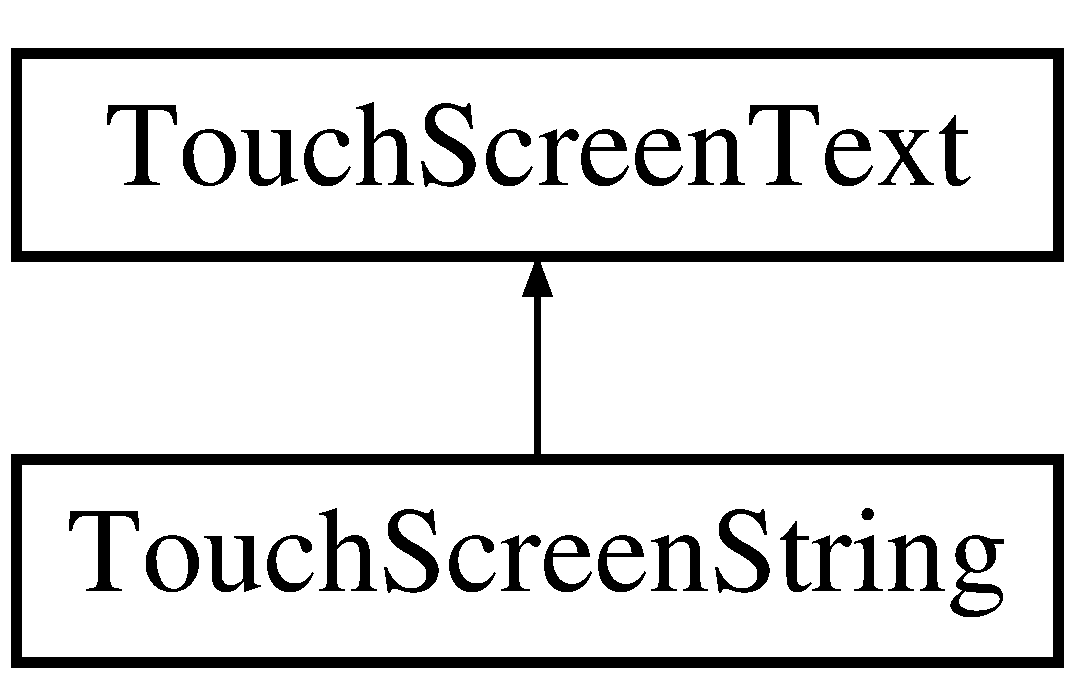
\includegraphics[height=2.000000cm]{class_touch_screen_string}
\end{center}
\end{figure}
\subsection*{Public Member Functions}
\begin{DoxyCompactItemize}
\item 
\hyperlink{class_touch_screen_string_ac6041c6c845b2286efee96cbc4b5473f}{Touch\+Screen\+String} ()
\begin{DoxyCompactList}\small\item\em Default constructor for the \hyperlink{class_touch_screen_string}{Touch\+Screen\+String} subclass. \end{DoxyCompactList}\item 
\hyperlink{class_touch_screen_string_a32ccd512fd5ef6a1aefa14d1e7552afb}{Touch\+Screen\+String} (\hyperlink{class_touch_screen_string}{Touch\+Screen\+String} \&other\+Touch\+Screen\+String)
\begin{DoxyCompactList}\small\item\em Copy constructor for the \hyperlink{class_touch_screen_string}{Touch\+Screen\+String} superclass. \end{DoxyCompactList}\item 
\hyperlink{class_touch_screen_string_a225634c4816f8988343c9a9491cf27fb}{Touch\+Screen\+String} (char $\ast$my\+Text, int my\+X\+Start, int my\+Y\+Start, int my\+Font\+Size, unsigned int my\+Text\+Color)
\begin{DoxyCompactList}\small\item\em Parameter constructor for the \hyperlink{class_touch_screen_string}{Touch\+Screen\+String} superclass. \end{DoxyCompactList}\item 
void \hyperlink{class_touch_screen_string_ad797bc5369aaace58de46bca39ae83dd}{set\+Values} (char $\ast$my\+Text, int my\+X\+Start, int my\+Y\+Start, int my\+Font\+Size, unsigned int my\+Text\+Color)
\begin{DoxyCompactList}\small\item\em Sets the text, coordinates, font size, and text color of the instance. \end{DoxyCompactList}\item 
void \hyperlink{class_touch_screen_string_a7d32e2262e4ea1009b029c0ae8b45897}{set\+Text} (char $\ast$)
\begin{DoxyCompactList}\small\item\em Sets the text of the string instance. \end{DoxyCompactList}\item 
const char $\ast$ \hyperlink{class_touch_screen_string_aadd13b945c6567a321a73f9e4220ee73}{get\+Text} ()
\begin{DoxyCompactList}\small\item\em Returns the text of the string instace. \end{DoxyCompactList}\item 
\hypertarget{class_touch_screen_string_a31873d10d7c6d9905048b76b969fa978}{void \hyperlink{class_touch_screen_string_a31873d10d7c6d9905048b76b969fa978}{draw\+Text} ()}\label{class_touch_screen_string_a31873d10d7c6d9905048b76b969fa978}

\begin{DoxyCompactList}\small\item\em Uses the T\+F\+T library to draw the string instance. \end{DoxyCompactList}\item 
void \hyperlink{class_touch_screen_string_a56d10098496bd88e0c60daf543447576}{text\+Button\+Display} ()
\begin{DoxyCompactList}\small\item\em Highlights the button text when pressed. \end{DoxyCompactList}\end{DoxyCompactItemize}
\subsection*{Additional Inherited Members}


\subsection{Detailed Description}
Subclass of \hyperlink{class_touch_screen_text}{Touch\+Screen\+Text}. Abstract class for drawing strings to the touch screen. 

\subsection{Constructor \& Destructor Documentation}
\hypertarget{class_touch_screen_string_ac6041c6c845b2286efee96cbc4b5473f}{\index{Touch\+Screen\+String@{Touch\+Screen\+String}!Touch\+Screen\+String@{Touch\+Screen\+String}}
\index{Touch\+Screen\+String@{Touch\+Screen\+String}!Touch\+Screen\+String@{Touch\+Screen\+String}}
\subsubsection[{Touch\+Screen\+String}]{\setlength{\rightskip}{0pt plus 5cm}Touch\+Screen\+String\+::\+Touch\+Screen\+String (
\begin{DoxyParamCaption}
{}
\end{DoxyParamCaption}
)}}\label{class_touch_screen_string_ac6041c6c845b2286efee96cbc4b5473f}


Default constructor for the \hyperlink{class_touch_screen_string}{Touch\+Screen\+String} subclass. 


\begin{DoxyParams}{Parameters}
{\em text} & The text that is to be drawn. \\
\hline
\end{DoxyParams}
\hypertarget{class_touch_screen_string_a32ccd512fd5ef6a1aefa14d1e7552afb}{\index{Touch\+Screen\+String@{Touch\+Screen\+String}!Touch\+Screen\+String@{Touch\+Screen\+String}}
\index{Touch\+Screen\+String@{Touch\+Screen\+String}!Touch\+Screen\+String@{Touch\+Screen\+String}}
\subsubsection[{Touch\+Screen\+String}]{\setlength{\rightskip}{0pt plus 5cm}Touch\+Screen\+String\+::\+Touch\+Screen\+String (
\begin{DoxyParamCaption}
\item[{{\bf Touch\+Screen\+String} \&}]{other\+Touch\+Screen\+String}
\end{DoxyParamCaption}
)}}\label{class_touch_screen_string_a32ccd512fd5ef6a1aefa14d1e7552afb}


Copy constructor for the \hyperlink{class_touch_screen_string}{Touch\+Screen\+String} superclass. 


\begin{DoxyParams}{Parameters}
{\em other\+Touch\+Screen\+String} & The string instance that is to be copied. \\
\hline
\end{DoxyParams}
\hypertarget{class_touch_screen_string_a225634c4816f8988343c9a9491cf27fb}{\index{Touch\+Screen\+String@{Touch\+Screen\+String}!Touch\+Screen\+String@{Touch\+Screen\+String}}
\index{Touch\+Screen\+String@{Touch\+Screen\+String}!Touch\+Screen\+String@{Touch\+Screen\+String}}
\subsubsection[{Touch\+Screen\+String}]{\setlength{\rightskip}{0pt plus 5cm}Touch\+Screen\+String\+::\+Touch\+Screen\+String (
\begin{DoxyParamCaption}
\item[{char $\ast$}]{my\+Text, }
\item[{int}]{my\+X\+Start, }
\item[{int}]{my\+Y\+Start, }
\item[{int}]{my\+Font\+Size, }
\item[{unsigned int}]{my\+Text\+Color}
\end{DoxyParamCaption}
)}}\label{class_touch_screen_string_a225634c4816f8988343c9a9491cf27fb}


Parameter constructor for the \hyperlink{class_touch_screen_string}{Touch\+Screen\+String} superclass. 


\begin{DoxyParams}{Parameters}
{\em my\+Text} & The text that is to be drawn. \\
\hline
{\em my\+X\+Start} & The x-\/coordinate for the text instance. \\
\hline
{\em my\+Y\+Start} & The y-\/coordinate for the text instance. \\
\hline
{\em my\+Font\+Size} & The font size of the text instance. \\
\hline
{\em my\+Text\+Color} & The color of the text instance. \\
\hline
\end{DoxyParams}


\subsection{Member Function Documentation}
\hypertarget{class_touch_screen_string_aadd13b945c6567a321a73f9e4220ee73}{\index{Touch\+Screen\+String@{Touch\+Screen\+String}!get\+Text@{get\+Text}}
\index{get\+Text@{get\+Text}!Touch\+Screen\+String@{Touch\+Screen\+String}}
\subsubsection[{get\+Text}]{\setlength{\rightskip}{0pt plus 5cm}const char $\ast$ Touch\+Screen\+String\+::get\+Text (
\begin{DoxyParamCaption}
{}
\end{DoxyParamCaption}
)}}\label{class_touch_screen_string_aadd13b945c6567a321a73f9e4220ee73}


Returns the text of the string instace. 

\begin{DoxyReturn}{Returns}
text The text that is to be drawn. 
\end{DoxyReturn}
\hypertarget{class_touch_screen_string_a7d32e2262e4ea1009b029c0ae8b45897}{\index{Touch\+Screen\+String@{Touch\+Screen\+String}!set\+Text@{set\+Text}}
\index{set\+Text@{set\+Text}!Touch\+Screen\+String@{Touch\+Screen\+String}}
\subsubsection[{set\+Text}]{\setlength{\rightskip}{0pt plus 5cm}void Touch\+Screen\+String\+::set\+Text (
\begin{DoxyParamCaption}
\item[{char $\ast$}]{my\+Text}
\end{DoxyParamCaption}
)}}\label{class_touch_screen_string_a7d32e2262e4ea1009b029c0ae8b45897}


Sets the text of the string instance. 


\begin{DoxyParams}{Parameters}
{\em my\+Text} & The text that is to be drawn. \\
\hline
\end{DoxyParams}
\hypertarget{class_touch_screen_string_ad797bc5369aaace58de46bca39ae83dd}{\index{Touch\+Screen\+String@{Touch\+Screen\+String}!set\+Values@{set\+Values}}
\index{set\+Values@{set\+Values}!Touch\+Screen\+String@{Touch\+Screen\+String}}
\subsubsection[{set\+Values}]{\setlength{\rightskip}{0pt plus 5cm}void Touch\+Screen\+String\+::set\+Values (
\begin{DoxyParamCaption}
\item[{char $\ast$}]{my\+Text, }
\item[{int}]{my\+X\+Start, }
\item[{int}]{my\+Y\+Start, }
\item[{int}]{my\+Font\+Size, }
\item[{unsigned int}]{my\+Text\+Color}
\end{DoxyParamCaption}
)}}\label{class_touch_screen_string_ad797bc5369aaace58de46bca39ae83dd}


Sets the text, coordinates, font size, and text color of the instance. 


\begin{DoxyParams}{Parameters}
{\em my\+Text} & The text that is to be drawn. \\
\hline
{\em my\+X\+Start} & The x-\/coordinate for the text instance. \\
\hline
{\em my\+Y\+Start} & The y-\/coordinate for the text instance. \\
\hline
{\em my\+Font\+Size} & The font size of the text instance. \\
\hline
{\em my\+Text\+Color} & The color of the text instance. Default color is W\+H\+I\+T\+E. \\
\hline
\end{DoxyParams}
\hypertarget{class_touch_screen_string_a56d10098496bd88e0c60daf543447576}{\index{Touch\+Screen\+String@{Touch\+Screen\+String}!text\+Button\+Display@{text\+Button\+Display}}
\index{text\+Button\+Display@{text\+Button\+Display}!Touch\+Screen\+String@{Touch\+Screen\+String}}
\subsubsection[{text\+Button\+Display}]{\setlength{\rightskip}{0pt plus 5cm}void Touch\+Screen\+String\+::text\+Button\+Display (
\begin{DoxyParamCaption}
{}
\end{DoxyParamCaption}
)}}\label{class_touch_screen_string_a56d10098496bd88e0c60daf543447576}


Highlights the button text when pressed. 

$<$ Sets the color to red

$<$ Sets the color to white 

The documentation for this class was generated from the following files\+:\begin{DoxyCompactItemize}
\item 
Touch\+Screen\+Strings.\+h\item 
Touch\+Screen\+Strings.\+cpp\end{DoxyCompactItemize}

\hypertarget{class_touch_screen_text}{\section{Touch\+Screen\+Text Class Reference}
\label{class_touch_screen_text}\index{Touch\+Screen\+Text@{Touch\+Screen\+Text}}
}


Base class for drawing text to the touch screen.  




{\ttfamily \#include $<$Touch\+Screen\+Strings.\+h$>$}

Inheritance diagram for Touch\+Screen\+Text\+:\begin{figure}[H]
\begin{center}
\leavevmode
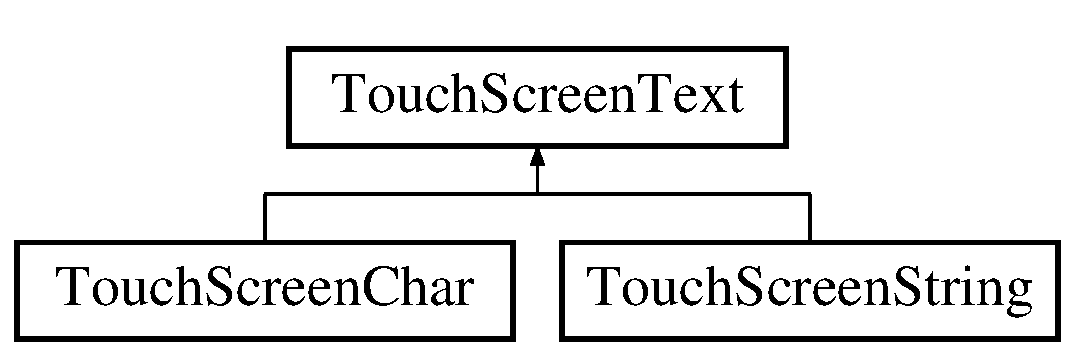
\includegraphics[height=2.000000cm]{class_touch_screen_text}
\end{center}
\end{figure}
\subsection*{Public Member Functions}
\begin{DoxyCompactItemize}
\item 
\hypertarget{class_touch_screen_text_ab4eb34ba6e6d41dbcbc00377f497efb8}{\hyperlink{class_touch_screen_text_ab4eb34ba6e6d41dbcbc00377f497efb8}{Touch\+Screen\+Text} ()}\label{class_touch_screen_text_ab4eb34ba6e6d41dbcbc00377f497efb8}

\begin{DoxyCompactList}\small\item\em Default constructor for the \hyperlink{class_touch_screen_text}{Touch\+Screen\+Text} superclass. \end{DoxyCompactList}\item 
\hypertarget{class_touch_screen_text_ab1d335963b16d5c06182002d32b485dc}{{\bfseries Touch\+Screen\+Text} (\hyperlink{class_touch_screen_text}{Touch\+Screen\+Text} \&other\+Touch\+Screen\+Text)}\label{class_touch_screen_text_ab1d335963b16d5c06182002d32b485dc}

\item 
\hyperlink{class_touch_screen_text_a4603c93a9419c4a7ab81b24d7a925a7b}{Touch\+Screen\+Text} (int, int, int, unsigned int)
\begin{DoxyCompactList}\small\item\em Parameter constructor for the \hyperlink{class_touch_screen_text}{Touch\+Screen\+Text} superclass. \end{DoxyCompactList}\item 
void \hyperlink{class_touch_screen_text_ad93fb5b78ee2578fe3730210ba172ee7}{set\+Text\+Coord} (int, int)
\begin{DoxyCompactList}\small\item\em Sets the coordinates of the text. \end{DoxyCompactList}\item 
void \hyperlink{class_touch_screen_text_ab276b0e4f90739d052e521d0e2fe5cc2}{set\+Font\+Size} (int my\+Font\+Size=2)
\begin{DoxyCompactList}\small\item\em Sets the font size of the text. \end{DoxyCompactList}\item 
void \hyperlink{class_touch_screen_text_a5a1bbd3e035ec114da0a341dad341461}{set\+Text\+Color} (unsigned int my\+Text\+Color=0xffff)
\begin{DoxyCompactList}\small\item\em Sets the color of the text. \end{DoxyCompactList}\item 
const int \hyperlink{class_touch_screen_text_ad4bf2d307ed2c96eed40969cdbdf4bcc}{get\+X\+Start} ()
\begin{DoxyCompactList}\small\item\em Gets the xcoordinate of the text. \end{DoxyCompactList}\item 
const int \hyperlink{class_touch_screen_text_a50372422c5ddb6c9b9f689a1e95e92ae}{get\+Y\+Start} ()
\begin{DoxyCompactList}\small\item\em Gets the ycoordinate of the text. \end{DoxyCompactList}\item 
const int \hyperlink{class_touch_screen_text_a34115eeb243b200e8546d7b203e8be54}{get\+Font\+Size} ()
\begin{DoxyCompactList}\small\item\em Gets the font size of the text. \end{DoxyCompactList}\item 
const int \hyperlink{class_touch_screen_text_ab1ba5d5526f00d925e5b0239901b7d50}{get\+Text\+Color} ()
\begin{DoxyCompactList}\small\item\em Gets the font color of the text. \end{DoxyCompactList}\end{DoxyCompactItemize}
\subsection*{Protected Attributes}
\begin{DoxyCompactItemize}
\item 
\hypertarget{class_touch_screen_text_af22a7ca72947722e7ff76ec0750dc851}{int {\bfseries xstart}}\label{class_touch_screen_text_af22a7ca72947722e7ff76ec0750dc851}

\item 
\hypertarget{class_touch_screen_text_a779b5c6ee8be737c4fbfc7ad002c5854}{int {\bfseries ystart}}\label{class_touch_screen_text_a779b5c6ee8be737c4fbfc7ad002c5854}

\item 
\hypertarget{class_touch_screen_text_a098422c325ce23c6d28d2b72ffb52a1a}{int \hyperlink{class_touch_screen_text_a098422c325ce23c6d28d2b72ffb52a1a}{font\+Size}}\label{class_touch_screen_text_a098422c325ce23c6d28d2b72ffb52a1a}

\begin{DoxyCompactList}\small\item\em Coordinates of the text. \end{DoxyCompactList}\item 
\hypertarget{class_touch_screen_text_a0b555c473dff7436a79c836926235217}{unsigned int \hyperlink{class_touch_screen_text_a0b555c473dff7436a79c836926235217}{text\+Color}}\label{class_touch_screen_text_a0b555c473dff7436a79c836926235217}

\begin{DoxyCompactList}\small\item\em Size of the text. \end{DoxyCompactList}\end{DoxyCompactItemize}


\subsection{Detailed Description}
Base class for drawing text to the touch screen. 

Parameter constructor for the \hyperlink{class_touch_screen_text}{Touch\+Screen\+Text} superclass.


\begin{DoxyParams}{Parameters}
{\em other\+Touch\+Screen\+Text} & The text that is to be copied. \\
\hline
\end{DoxyParams}


\subsection{Constructor \& Destructor Documentation}
\hypertarget{class_touch_screen_text_a4603c93a9419c4a7ab81b24d7a925a7b}{\index{Touch\+Screen\+Text@{Touch\+Screen\+Text}!Touch\+Screen\+Text@{Touch\+Screen\+Text}}
\index{Touch\+Screen\+Text@{Touch\+Screen\+Text}!Touch\+Screen\+Text@{Touch\+Screen\+Text}}
\subsubsection[{Touch\+Screen\+Text}]{\setlength{\rightskip}{0pt plus 5cm}Touch\+Screen\+Text\+::\+Touch\+Screen\+Text (
\begin{DoxyParamCaption}
\item[{int}]{my\+X\+Start, }
\item[{int}]{my\+Y\+Start, }
\item[{int}]{my\+Font\+Size, }
\item[{unsigned int}]{my\+Text\+Color}
\end{DoxyParamCaption}
)}}\label{class_touch_screen_text_a4603c93a9419c4a7ab81b24d7a925a7b}


Parameter constructor for the \hyperlink{class_touch_screen_text}{Touch\+Screen\+Text} superclass. 


\begin{DoxyParams}{Parameters}
{\em my\+X\+Start} & The x-\/coordinate for the text instance. \\
\hline
{\em my\+Y\+Start} & The y-\/coordinate for the text instance. \\
\hline
{\em my\+Font\+Size} & The font size of the text instance. \\
\hline
{\em my\+Text\+Color} & The color of the text instance. Default color is W\+H\+I\+T\+E. \\
\hline
\end{DoxyParams}


\subsection{Member Function Documentation}
\hypertarget{class_touch_screen_text_a34115eeb243b200e8546d7b203e8be54}{\index{Touch\+Screen\+Text@{Touch\+Screen\+Text}!get\+Font\+Size@{get\+Font\+Size}}
\index{get\+Font\+Size@{get\+Font\+Size}!Touch\+Screen\+Text@{Touch\+Screen\+Text}}
\subsubsection[{get\+Font\+Size}]{\setlength{\rightskip}{0pt plus 5cm}const int Touch\+Screen\+Text\+::get\+Font\+Size (
\begin{DoxyParamCaption}
{}
\end{DoxyParamCaption}
)}}\label{class_touch_screen_text_a34115eeb243b200e8546d7b203e8be54}


Gets the font size of the text. 

\begin{DoxyReturn}{Returns}
The font size for the text instance. 
\end{DoxyReturn}
\hypertarget{class_touch_screen_text_ab1ba5d5526f00d925e5b0239901b7d50}{\index{Touch\+Screen\+Text@{Touch\+Screen\+Text}!get\+Text\+Color@{get\+Text\+Color}}
\index{get\+Text\+Color@{get\+Text\+Color}!Touch\+Screen\+Text@{Touch\+Screen\+Text}}
\subsubsection[{get\+Text\+Color}]{\setlength{\rightskip}{0pt plus 5cm}const int Touch\+Screen\+Text\+::get\+Text\+Color (
\begin{DoxyParamCaption}
{}
\end{DoxyParamCaption}
)}}\label{class_touch_screen_text_ab1ba5d5526f00d925e5b0239901b7d50}


Gets the font color of the text. 

\begin{DoxyReturn}{Returns}
The font color for the text instance. 
\end{DoxyReturn}
\hypertarget{class_touch_screen_text_ad4bf2d307ed2c96eed40969cdbdf4bcc}{\index{Touch\+Screen\+Text@{Touch\+Screen\+Text}!get\+X\+Start@{get\+X\+Start}}
\index{get\+X\+Start@{get\+X\+Start}!Touch\+Screen\+Text@{Touch\+Screen\+Text}}
\subsubsection[{get\+X\+Start}]{\setlength{\rightskip}{0pt plus 5cm}const int Touch\+Screen\+Text\+::get\+X\+Start (
\begin{DoxyParamCaption}
{}
\end{DoxyParamCaption}
)}}\label{class_touch_screen_text_ad4bf2d307ed2c96eed40969cdbdf4bcc}


Gets the xcoordinate of the text. 

\begin{DoxyReturn}{Returns}
The x-\/coordinate for the text instance. 
\end{DoxyReturn}
\hypertarget{class_touch_screen_text_a50372422c5ddb6c9b9f689a1e95e92ae}{\index{Touch\+Screen\+Text@{Touch\+Screen\+Text}!get\+Y\+Start@{get\+Y\+Start}}
\index{get\+Y\+Start@{get\+Y\+Start}!Touch\+Screen\+Text@{Touch\+Screen\+Text}}
\subsubsection[{get\+Y\+Start}]{\setlength{\rightskip}{0pt plus 5cm}const int Touch\+Screen\+Text\+::get\+Y\+Start (
\begin{DoxyParamCaption}
{}
\end{DoxyParamCaption}
)}}\label{class_touch_screen_text_a50372422c5ddb6c9b9f689a1e95e92ae}


Gets the ycoordinate of the text. 

\begin{DoxyReturn}{Returns}
The y-\/coordinate for the text instance. 
\end{DoxyReturn}
\hypertarget{class_touch_screen_text_ab276b0e4f90739d052e521d0e2fe5cc2}{\index{Touch\+Screen\+Text@{Touch\+Screen\+Text}!set\+Font\+Size@{set\+Font\+Size}}
\index{set\+Font\+Size@{set\+Font\+Size}!Touch\+Screen\+Text@{Touch\+Screen\+Text}}
\subsubsection[{set\+Font\+Size}]{\setlength{\rightskip}{0pt plus 5cm}void Touch\+Screen\+Text\+::set\+Font\+Size (
\begin{DoxyParamCaption}
\item[{int}]{my\+Font\+Size = {\ttfamily 2}}
\end{DoxyParamCaption}
)}}\label{class_touch_screen_text_ab276b0e4f90739d052e521d0e2fe5cc2}


Sets the font size of the text. 


\begin{DoxyParams}{Parameters}
{\em my\+Font\+Size} & The font size of the text instance. \\
\hline
\end{DoxyParams}
\hypertarget{class_touch_screen_text_a5a1bbd3e035ec114da0a341dad341461}{\index{Touch\+Screen\+Text@{Touch\+Screen\+Text}!set\+Text\+Color@{set\+Text\+Color}}
\index{set\+Text\+Color@{set\+Text\+Color}!Touch\+Screen\+Text@{Touch\+Screen\+Text}}
\subsubsection[{set\+Text\+Color}]{\setlength{\rightskip}{0pt plus 5cm}void Touch\+Screen\+Text\+::set\+Text\+Color (
\begin{DoxyParamCaption}
\item[{unsigned int}]{my\+Text\+Color = {\ttfamily 0xffff}}
\end{DoxyParamCaption}
)}}\label{class_touch_screen_text_a5a1bbd3e035ec114da0a341dad341461}


Sets the color of the text. 


\begin{DoxyParams}{Parameters}
{\em my\+Text\+Color} & The color of the text instance. \\
\hline
\end{DoxyParams}
\hypertarget{class_touch_screen_text_ad93fb5b78ee2578fe3730210ba172ee7}{\index{Touch\+Screen\+Text@{Touch\+Screen\+Text}!set\+Text\+Coord@{set\+Text\+Coord}}
\index{set\+Text\+Coord@{set\+Text\+Coord}!Touch\+Screen\+Text@{Touch\+Screen\+Text}}
\subsubsection[{set\+Text\+Coord}]{\setlength{\rightskip}{0pt plus 5cm}void Touch\+Screen\+Text\+::set\+Text\+Coord (
\begin{DoxyParamCaption}
\item[{int}]{my\+X\+Start, }
\item[{int}]{my\+Y\+Start}
\end{DoxyParamCaption}
)}}\label{class_touch_screen_text_ad93fb5b78ee2578fe3730210ba172ee7}


Sets the coordinates of the text. 


\begin{DoxyParams}{Parameters}
{\em my\+X\+Start} & The x-\/coordinate for the text instance. \\
\hline
{\em my\+Y\+Start} & The y-\/coordinate for the text instance. \\
\hline
\end{DoxyParams}


The documentation for this class was generated from the following files\+:\begin{DoxyCompactItemize}
\item 
Touch\+Screen\+Strings.\+h\item 
Touch\+Screen\+Strings.\+cpp\end{DoxyCompactItemize}

%--- End generated contents ---

% Index
\newpage
\phantomsection
\addcontentsline{toc}{chapter}{Index}
\printindex

\end{document}
